\chapter{Resultados}
\label{chap:result}
Aqui trataremos sobre os resultados que foram encontrados durante o desenvolvimentodo projeto. Foi um projeto extenso e com dificuldades em certos momentos, porém, no fim conseguimos conclui-lo e trazer os resultados deste projeto à tona.


\section{Diagrama de classes}
\label{sec:class}
O diagrama de classes é uma representação visual das classes do sistema e seus relacionamentos. 
\begin{figure} [h!]	
    \centering
    \caption{Meu diagrama de classes}
    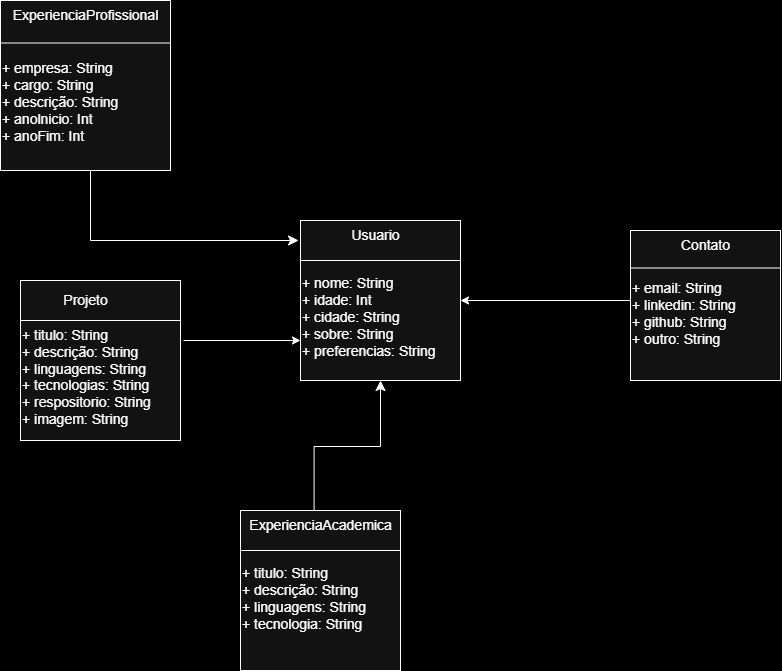
\includegraphics[width=0.8\textwidth]{Figures/diagrama-de-classes.png}
    \caption*{Fonte: Autoria própria.}
    \label{fig:diagrama_classes}
\end{figure}

favor olhar a seção \ref{sec:class}.


\section{Diagrama de casos de uso}
\label{sec:casos}
O diagrama de casos de uso é uma representação visual dos casos de uso do sistema e os atores envolvidos. Ele é utilizado para descrever as funcionalidades do sistema e como os usuários interagem com ele. A Figura \ref{fig:diagrama_casos} apresenta o diagrama de casos de uso do projeto desenvolvido.
\begin{figure} [h!]	
    \centering
    \caption{Meu diagrama de casos de uso}
    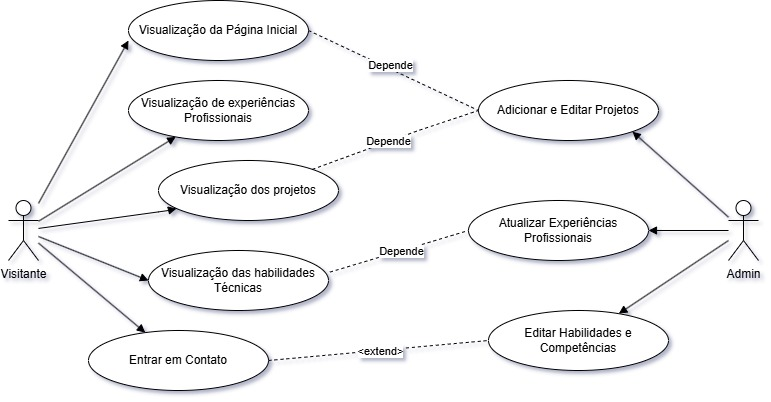
\includegraphics[width=0.8\textwidth]{Figures/diagrama-casos-de-uso.jpeg}
    \caption*{Fonte: Autoria própria.}
    \label{fig:diagrama_casos}
\end{figure}


\section{Diagrama de sequência}
\label{sec:sequencia}   
O diagrama de sequência é uma representação visual da interação entre os objetos do sistema ao longo do tempo. Ele é utilizado para descrever como os objetos interagem entre si para realizar uma determinada funcionalidade. A Figura \ref{fig:diagrama_sequencia} apresenta o diagrama de sequência do projeto desenvolvido. 
\begin{figure} [h!]	
    \centering
    \caption{Meu diagrama de sequencia}
    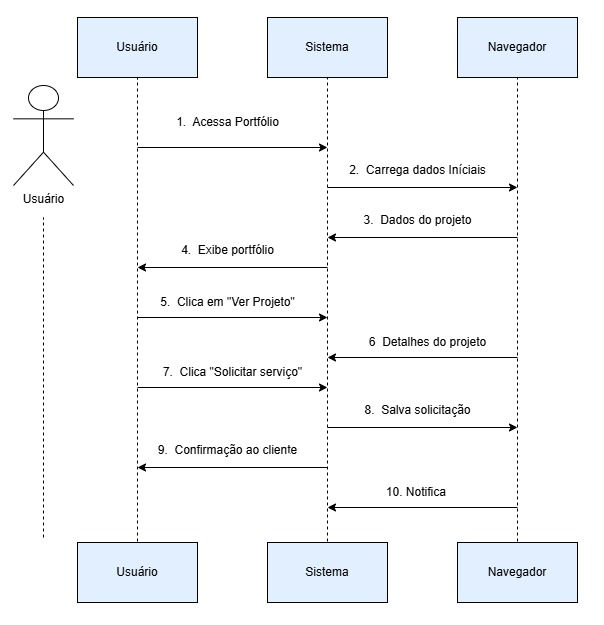
\includegraphics[width=0.8\textwidth]{Figures/diagrama-de-sequencia.jpeg}
    \caption*{Fonte: Autoria própria.}
    \label{fig:diagrama_sequencia}
\end{figure}







